\documentclass[twoside]{article}
\usepackage{exam}
\usepackage{multicol}
\usepackage[export]{adjustbox}

\pagestyle{myheadings}
\markboth{}{{\large Name: }\sp{4in}}
\nonstopmode

% For Python code
\lstset{%
  language=Python,
  basicstyle=\ttfamily,
  showstringspaces=false
  keywordstyle=\color{black},
  commentstyle=\color{black},
  stringstyle=\color{black},
}

\newcommand{\bubble}{\raisebox{-0.3ex}{
\includegraphics[height=2ex]{oval.png}}}
\newcommand{\filledbubble}{\raisebox{-0.3ex}{
\includegraphics[height=2ex]{oval-filled.png}}}

%%% Showing solutions %%%%%%%%%%%%%%%%%%%%%%%%%%%%%%%%%%%%%%%%%%%%%%%%%%%%%%%%%


% \newcommand{\solution}[1]{{\color{red}#1}}
\newcommand\solution[1]{} % excludes

\newcommand{\solutioncircle}[1]{{\color{red}#1}}
% \newcommand{\solutioncircle}[1]{#1} % don't color text but still display it

\newcommand{\solutionimage}[2]{#2}  % First arg is question, second is solution
% \newcommand{\solutionimage}[2]{#1} % First arg is question, second is solution

\newcommand{\versioned}[2]{#1} % First arg is question, second is solution
% \newcommand{\versioned}[2]{#2} % First arg is question, second is solution

%%% Document %%%%%%%%%%%%%%%%%%%%%%%%%%%%%%%%%%%%%%%%%%%%%%%%%%%%%%%%%%%%%%%%%%

\title{\sc Final \solution{Solutions}}

\begin{document}
\thispagestyle{empty}
\maketitle

\medskip

\textbf{INSTRUCTIONS}

\begin{itemize}
\item You have 2 hours and 50 minutes to complete the exam.

\item The exam is closed book, closed notes, closed computer, closed calculator,
except for the official reference guide provided with the exam.

\item Mark your answers \textbf{on the exam itself}. We will \emph{not} grade
answers written on scratch paper.

\item You may leave numerical calculations unsimplified throughout the exam.

\item You may assume that the statements {\tt import numpy as np} and {\tt from datascience import *} have been executed throughout the exam.

\item No questions will be allowed during the time of the final. If something is unclear, you may state an assumption. If the assumption is valid, we will grade based on your assumption. 
\end{itemize}
\textbf{Question 0 (1 point)} Write your name in the space provided on one side of every page of the exam. 
\medskip

\begin{center}
\begin{tabular}{|m{6cm}|m{8cm}|}
\hline
Last name & \\ [1cm]
\hline
First name & \\ [1cm]
\hline
Email & \\ [1cm]
\hline
Name of the person to your left & \\ [1cm]
\hline
Name of the person to your right & \\ [1cm]
\hline
\emph{All the work on this exam is my own.} \textbf{(please sign)} & \\ [1cm]
\hline
\end{tabular}
\end{center}
\vfill
\vfill
\newpage
% \center{This page was intentionally left blank.}
% \newpage

\begin{enumerate}
    \q{13}{YouTable} \\ 

You are interested in finding out who the most popular YouTube content producers in the United States are. Your colleague used the YouTube online statistics API to find out the top 250 YouTubers in the United States as of August 2018, based on total number of video views. The first few rows of her dataset {\tt yt} are shown below. 

\begin{center}
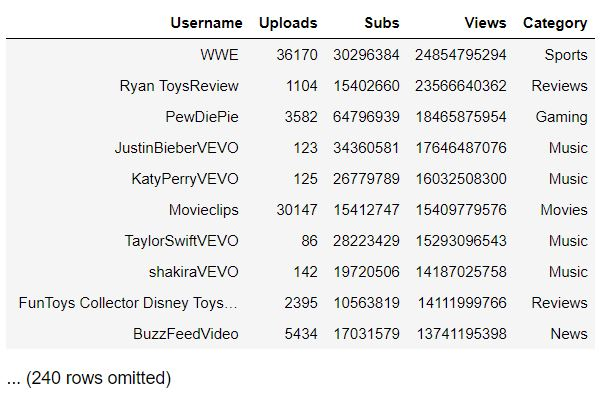
\includegraphics[scale=0.9]{yt_with_reviews.JPG}
\end{center}

In the table above, the entries in the columns \textbf{Username} and \textbf{Category} are of type {\tt string} while the entries in all other columns are of type {\tt int}. \textbf{Uploads} corresponds to number of video uploads per artist, \textbf{Subs} is number of active subscribers, and \textbf{Views} is total amount of views in all the videos a YouTube artist has released.

Fill in the blanks of the Python expressions to compute the described values. You must use only the lines provided to get full credit.The  last  line  of  each  answer  should  evaluate  to  the  value described.   Assume  that  the  statements {\tt import numpy as np} and {\tt from datascience import *} have  been executed.  You may enter anything you would like in the blanks below, but you may not add code outside of the blanks.

\begin{enumerate}

\subq{1} The total number of YouTubers in this table who have more than 1000 video uploads.\\

\lstinline{yt.________________________________________________________________________________} \\ \\
\solution{
\lstinline{yt.where('Uploads', are.above(1000)).num_rows}
}

\subq{2} You realize that the music video streaming platform VEVO contributes a lot of the top US YouTube artist accounts like "TaylorSwiftVEVO" and "shakiraVEVO". Create a table that only contains channels from VEVO, with the artists with the most subscribers at the top.\\

\lstinline{yt._________________________________________________________________________________} \\ \\
\solution{
\lstinline{yt.where('Username', are.containing('VEVO')).sort('Subs', descending=True)} \\ \\
}

\subq{3} You are interested in finding the category (ex. Sports, Music, News) with the largest average number of subscribers. Fill in the lines below so that the last line evaluates to said category.

\lstinline{only_sub_and_cat = yt.______________________________________________________________} \\ \\
\lstinline{only_sub_and_cat.___________________________________________________________________} \\ \\
\solution{
\lstinline{only_sub_and_cat = yt.select('Category', 'Subs')} \\ \\
\lstinline{only_sub_and_cat.group(0, np.mean).sort(1, descending = True).column(0).item(0)} \\ \\ 
Many people used take incorrectly. Remember take expects an array of row indicies to take from the table. 
}


\subq{3} Your friend proposes that a more effective popularity metric for YouTube content creators might be view count per video upload. Create a table with one column that contains only the usernames of the 5 top US YouTubers, sorted by highest view count per video upload.\\ \\
\lstinline{views_per_upload  = ____________________________________________________________________} \\ \\
\lstinline{yt_new_metric =  yt.with_column(________________________________________________________)} \\ \\
\lstinline{yt_new_metric.__________________________________________________________________________}\\ \\
\solution{
\lstinline{views_per_upload = yt.column('Views')/yt.column('Uploads')} \\ \\
\lstinline{yt_new_metric = yt.with_column('views_per_upload', views_per_upload)} \\ \\
\lstinline{yt_new_metric.sort('views_per_upload', descending=True).take(np.arange(5)).select('Username')}}
\\


In addition to the top 250 US YouTube accounts table from before, your friend finds a second table for the top 250 UK (United Kingdom) YouTube accounts, sorted by subscriber count. The first few rows of the {\tt yt\_uk} table are shown below. \\

\begin{center}
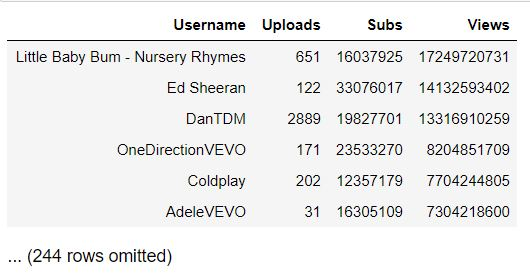
\includegraphics[scale=0.9]{youtubers_tbl_uk.JPG}
\end{center}

\subq{4} Find the number of YouTubers that are \textbf{only present in one} of the top 250 subscriber lists between the two countries. \\

\lstinline{num_youtubers_in_both =__________________________________________________________________} \\ \\
\lstinline{__________________________________________________________________________________________} \\ \\
\solution{
\lstinline{num_youtubers_in_both = yt_uk.join('Username', yt)} \\ \\
\lstinline{yt.num_rows + yt_uk.num_rows - 2*num_youtubers_in_both.num_rows} \\ \\
}
\end{enumerate}

    \q{10}{Spotify Shuffle}

Fahad creates a Spotify music playlist by randomly sampling 100 songs from a large collection of tunes from the Data 8 staff music library. It is known that staff library contains 20\% Hip-Hop songs, 35\% Pop songs, 15\% Rock songs, 25\% Dance songs, and 5\% Country songs. 

Vinitra notices that in Fahad's playlist, there are 30\% Hip-Hop songs, 30\% Pop songs, 20\% Rock songs, 18\% Dance songs, and 2\% Country songs. 

Initially, Vinitra believes that Fahad's claim that he randomly sampled 100 songs from the large staff library is false. Specifically, she believes he purposefully sampled more Hip-Hop songs. 
\begin{enumerate}
\subq{3} Describe a test statistic that we could compute given a sample that can help us pick between the two viewpoints: Fahad sampled the songs randomly and any difference is due to chance, or he was biased in his sampling technique and sampled more Hip-Hop songs. \\ \\ \\ \\ 
\solution{The percentage of songs that are Hip-Hop or the difference between actual number of hip hop songs and expected number of hip hop songs. TVD does not work because we specifically care if Hip Hop was higher than expected, not the whole distribution. Moreover, absolute value was incorrect because we care about a direction. }

\subq{2} Fill in the blank with the best number possible. No need to show your work. \\
If the null hypothesis was true, we expect our test statistic to be roughly equal to \underline{\hspace{3cm}}, and any difference in our sample is just due to random chance. \\ \\
\solution{20\% if your answer is percentage of hip hop songs above, or 0 otherwise. Your answer here depends on what you wrote on part a and was graded accordingly.} \\
Now, Vinitra decides that she does not care about Fahad's bias towards Hip-Hop. Instead, she simply does not believe that Fahad truly created his playlist by randomly sampling the 100 songs from the large staff library. She does not know how he sampled, but she believes it is not completely random. \\ 

\subq{3} Describe a test statistic that can help pick between the two viewpoints: Fahad sampled the songs randomly and any difference is due to chance, or he did not sample the songs randomly from the staff playlist.   \\ \\ \\ \\ 
\solution{The TVD between Fahad's claimed distribution of music genres and the sample that we obtain.}
\subq{2} Fill in the blank with the best number possible. No need to show your work. \\
If the null hypothesis was true, we expect our test statistic to be roughly equal to \underline{\hspace{3cm}}, and any difference in our sample is just due to random chance. \\ \\
\solution{0}
\end{enumerate}
    \q{8}{You're Samply Too Mean} 

The average weights of all people in California is 146 lb. Through some experimentation, we note that the probability of seeing a sample of 100 people (with replacement) in California whose average weight is higher than 151 lb is 2.5\%. 
\begin{enumerate}
\subq{4} Solve for the standard deviation of all weights in California. Show your work and box your final answer, which may be left unsimplified. \\ \\ \\ \\ \\ \\ \\ \\ \\ \\ \\ \\
\solution{If we have a 2.5\% chance of seeing an average sample weight higher than 146 lb, we know that is two standard deviations above the sample average distributions average (which is the population average weight), by the CLT. The SD of the sample means is PopSD / sqrt(Sample Size). In this case, we get that 2 * PopSD / 10 = 5. The PopSD is then 25. }
\subq{4} We would like to reduce the chance of seeing an average weight of a sample (drawn with replacement) that is higher than 151 lb to roughly .15\%. Solve for the smallest sample size which would achieve this goal. Show your work and box your final answer, which may be left unsimplified. Assume your answer to Part A is assigned to the variable $PopSD$ and use this variable in your final expression, if needed. \\ \\ \\ \\ \\ \\ \\
\solution{For 151 and above to represent .15\% of the data, that means 151 is 3 SDs above the sample mean (146). So, we want 5 to be 3 SDs of the sample mean. So, 3 * PopSD / sqrt(SampSize) = 5. Solving for Sample Size, we get $(3/5 * PopSD)^2$}
\newpage
\end{enumerate}




    \q{6}{Error Probabilities Probably} \\ 

A researcher conducts 1000 of the same hypothesis tests (same null, alternative, and test statistic) with different samples of observed data from a population. Throughout her hypothesis tests, she uses a p-value cutoff of .25. 
\\ \\
Suppose the following is a histogram of the p-values recorded during the conclusion for each of the 1000 hypothesis tests. The bin sizes are all a multiple of .05. 

\begin{center}
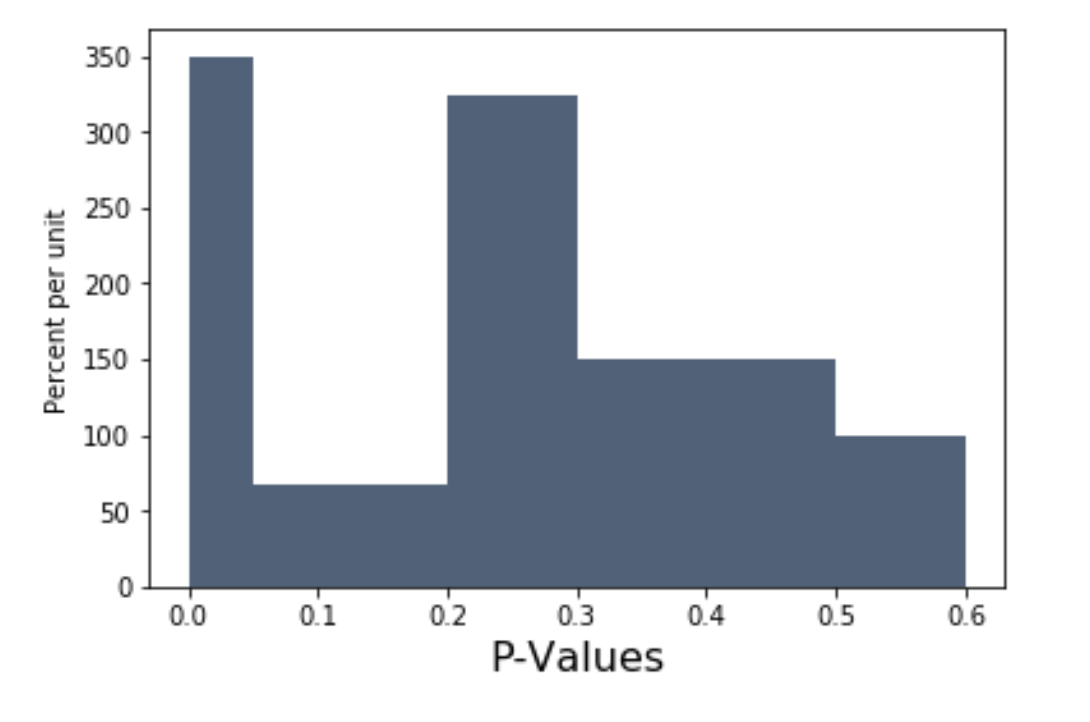
\includegraphics[scale=0.5]{phist.png}
\end{center}

\begin{enumerate}
\subq{3} Assume the null hypothesis in these tests happened to be true. If you can tell, did we reject the null hypothesis more than expected, less than expected, or exactly as many times as we would expect? \textbf{Explain} your answer. If we can not determine with this information, \textbf{explain} why not. 
\begin{itemize}[label=\bubble]
\item More than expected
\item Less than expected
\item Exactly equal to expected
\item Cannot determine
\end{itemize} 
\textbf{Explanation:}
\solution{
	Option 1. With a P-Value cut-off of 25\%, we expect to reject 25\% of all null hypotheses if they were indeed true. Here, we reject at-least $350 * .05 + 60 * .15$ which is greater than 25. 
}
\vfill

\subq{3} Assume the alternative hypothesis in these tests happened to be true. If you can tell, did we fail to reject the null hypothesis more than expected, less than expected, or exactly as many times as we would expect? \textbf{Explain} your answer. If we can not determine with this information, \textbf{explain} why not. 
\begin{itemize}[label=\bubble]
\item More than expected
\item Less than expected
\item Exactly equal to expected
\item Cannot determine
\end{itemize} 
\textbf{Explanation:}
\solution{Option 4. We have no information about anything assuming the alternative hypothesis was true because we never simulated anything under the alternative.}
\vfill
\end{enumerate}




    \newpage
    \q{19}{Linear Regret-ssion} \\

We are interested in seeing how the Per Capita Income was related with Infant Mortality rate for various countries in the early 1950s. The data is encapsulated in a table named {\tt countries}, whose first few rows are shown below: 

\begin{center}
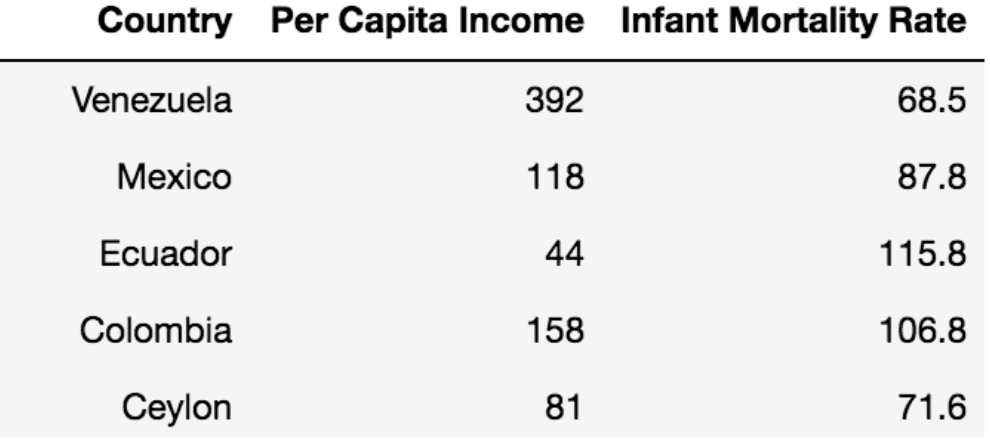
\includegraphics[scale=0.6]{regtable.png}
\end{center}

We are interested in looking at the relationship between Per Capita Income and Infant Mortality Rate. We plot two lines that we will use to predict infant mortality rate in a country (on average), given a per capita income. One is the regression line, and one is the constant line at the average of infant mortality rate. 

\begin{center}
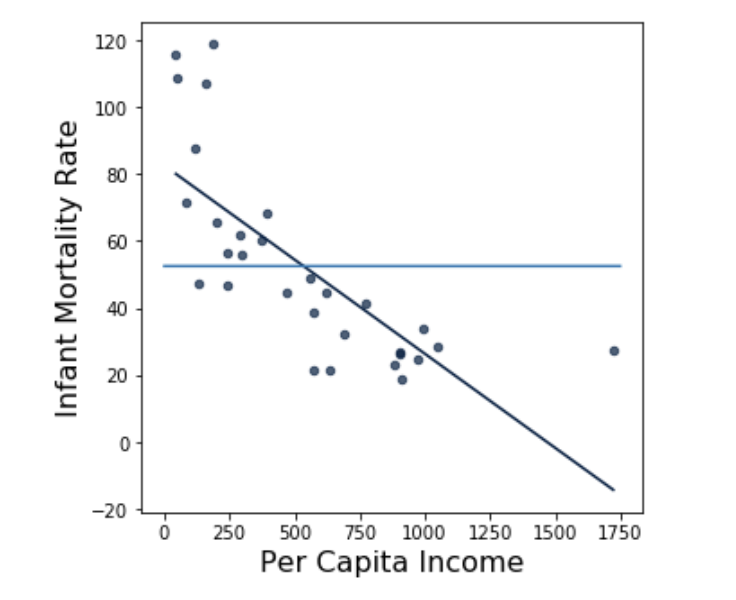
\includegraphics[scale=0.8]{regavg.png}
\end{center}

Here are some relevant lines of code and their outputs. Assume all of the functions below (descriptions of which appear on your study guide) are defined already. 

\begin{center}
 \begin{tabular}{||c c ||} 
 \hline
 Expression & Output\\ [0.5ex] 
 \hline\hline
 {\tt correlation(countries, 1, 2)} & -.74 \\ 
 \hline
 {\tt np.mean(countries.column(1))} & 534.1\\
 \hline
 {\tt np.mean(countries.column(2))} & 52.5\\
 \hline
 {\tt np.std(countries.column(1))} & 384.8\\
 \hline
 {\tt np.std(fitted\_values(countries, 1, 2))} & 21.6 \\ [1ex] 
 \hline
\end{tabular}
\end{center}


\begin{enumerate}

\subq{4} If possible, calculate the slope of the regression line in the plot above. Show your work with arithmetic. Please \textbf{do not} write any Python expressions. Box your final answer, which you may leave unsimplified. If it is not possible, explain why not. 
\\ \\ \\ \\ \\ \\ \\
\solution{Slope is r times the SD of y over SD of x. We have everything but SD of y. But, we can calculate that using the fact that we have the SD of the fitted values. The SD of the y is then $21.6 / .74$. We can then calculate for the slope using $r * \frac{SD(Y)}{SD(X)}$
}

\subq{2} At what value of per capita income would we predict the infant mortality rate to be 0 given the regression line on the previous page? 
\begin{itemize}[label=\bubble]
\item 0
\item 52.5
\item 80
\item 534.1
\item 1500
\item None of the above
\end{itemize} 
\solution{
	Option 5 -- based on graph
}



\subq{2} At what value of per capita income would we predict the infant mortality rate to be 0 given the average line on the previous page? 
\begin{itemize}[label=\bubble]
\item 0
\item 52.5
\item 80
\item 534.1
\item 1500
\item None of the above
\end{itemize} 
\solution{
	Option 6 -- based on graph 
} \\

\subq{3} Assume the RMSE (root mean squared error) of the regression line is 19.3. If possible, calculate the RMSE of the constant line representing the average of the infant mortality rate on this data. Show your work with arithmetic. Please \textbf{do not} write any Python expressions. Box your final answer, which you may leave unsimplified. If it is not possible, explain why not. \\ \\ \\ \\ \\ \\ \\
\solution{
The RMSE of the average line is actually just the SD of Infant Mortality Rate. We calculate that in Part a as $21.6 / .74$. 
}

\subq{3} If possible, fill in the blank with a mathematical expression. Box your final answer, which you may leave unsimplified. If it is not possible, explain why not. 
\\ \\ 
We use our regression line to estimate infant mortality rate using per capita income. At-least 88.9\% of our predictions of infant mortality rate will be correct within plus or minus \underline{\hspace{3cm}} units.
\solution{We notice that at least 88.9\% points us to three SDs both ways can be answered using Chebyshev's. We are trying to quantify the error, which is the residuals. So, we look at 3 SDs of the residuals both ways. We need to calculate the standard deviation of the residuals, which is $\sqrt{1-(-.74^2} * SD(Y)$. We calculated SD(Y) above, so our final answer is $3 * \sqrt{1 - .74**2} * 21.6 / .74$}

\\ \\
We move our attention to only the regression line and we would like to determine whether or not linear regression was a good idea to begin with. We show the regression line plotted on the scatter plot below again for convenience. \\
\begin{center}
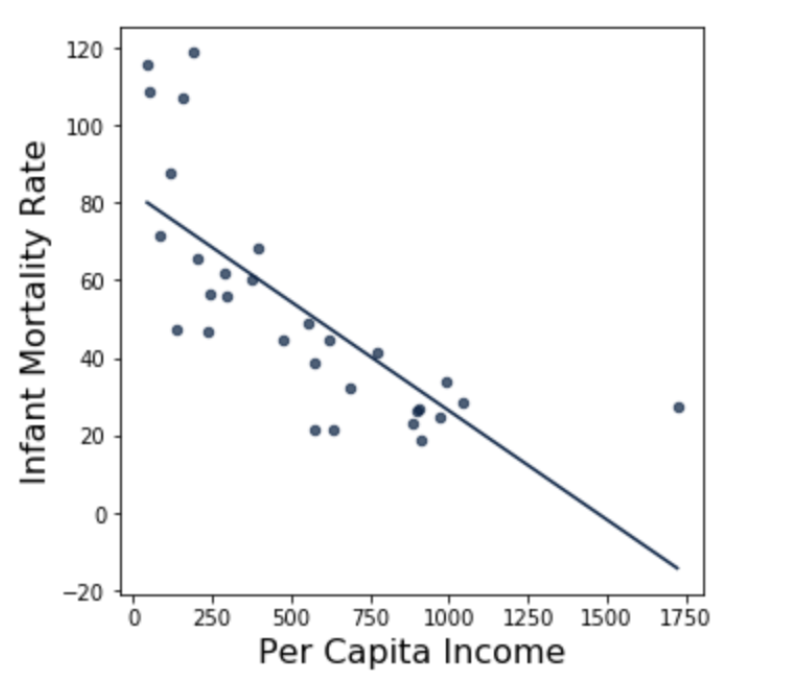
\includegraphics[scale=0.6]{regline.png}
\end{center} \\ \\
\subq{2} Which of the following plots is the best approximation to the residual plot, along with the line y=0?
\begin{multicols}{3}
\begin{itemize}[label=\bubble]
\item 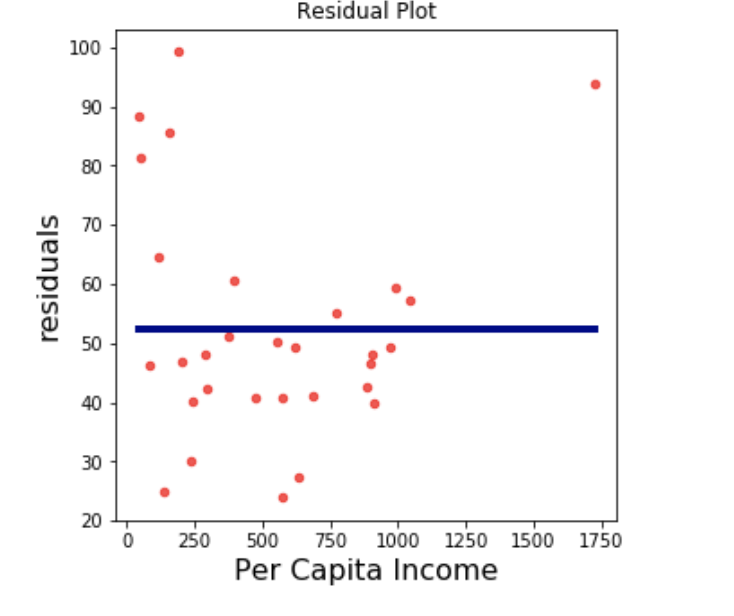
\includegraphics[scale=0.4]{resid2.png}
\item 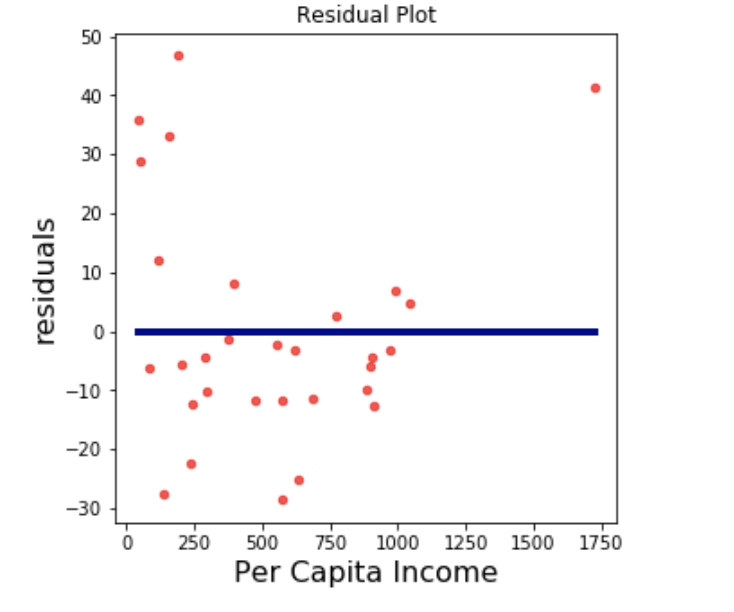
\includegraphics[scale=0.4]{resid1.png}
\item 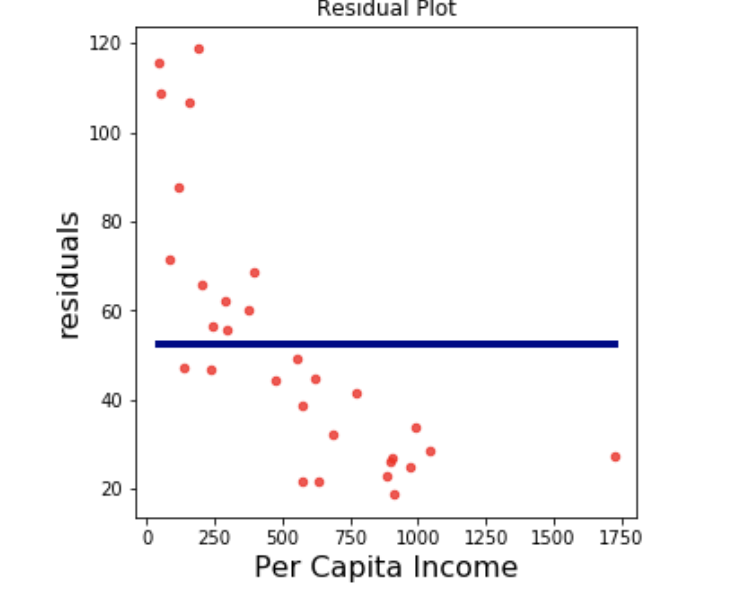
\includegraphics[scale=0.4]{resid3.png}
\end{itemize} 
\end{multicols}
\\ 
\solution{
	Option 2
}
\vfill

\subq{1} What is the approximate average value of the residuals? 
\begin{itemize}[label=\bubble]
\item -10
\item 0
\item 52.5
\item 534.1
\item Need more information
\end{itemize} 
\\ 
\solution{
	Option 2 -- Average of the residuals is always 0. 
}
\vfill
\subq{2} Based on the information above, select the most appropriate statement below. 
\begin{itemize}[label=\bubble]
\item Our residual plot shows no obvious pattern, so linear regression is a good fit for this data.
\item Our residual plot shows a definitive pattern, but based on our original plot, linear regression is still a good fit for this data.
\item Our residual plot shows a linearly decreasing trend, so linear regression is not a good fit for this data.
\item Our residual plot shows a definitive pattern, so linear regression is not a good fit for this data.
\item None of the above
\end{itemize} 
\\ 
\solution{
	Option 4 -- a pattern is present, but it is not decreasing linearly. It goes down, then comes back up. Since there is pattern in the residual plot, linear regression is not a good idea. 
}
\vfill



\end{enumerate}
    \newpage
    \q{18}{HA/Biness Among Countries} \\ 

We are interesting in studying the distribution of human happiness across the world. To do so, we have a table called {\tt happiness}. The table has 140 rows, and the first few rows are shown below: 

\begin{center}
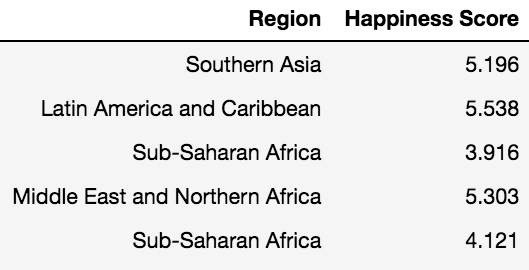
\includegraphics[scale=1]{countries.png}
\end{center}\\
\\ 
Each row contains the region and happiness score for a sampled country. The countries are not shown in the table above. Throughout this question, our goal will be to measure if the distribution of happiness scores across regions in the whole world are roughly equivalent. 

\begin{enumerate}
\subq{2} Define a function {\tt region\_happiness} which takes in a table like  {\tt happiness} and returns a two column table. The output table should have one column with the names of the unique regions, and a second column with the average happiness score in that region. The first few rows of an output table are shown below, with one row for each unique region. Note that the input table may not have the same labels as {\tt happiness}, but will have the same ordering of columns.

\begin{center}
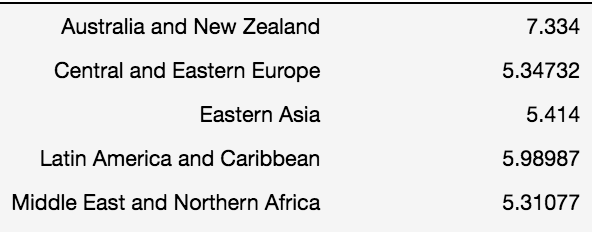
\includegraphics[scale=0.9]{regions.png}
\end{center}\\ \\ \\
 
\lstinline{def region_happiness(tbl):}\\ \\
\lstinline{     return ____________________________________________________________________________}
\\
\solution{
\lstinline{def region_happiness(tbl):}\\ \\
\lstinline{     return tbl.group(0, np.average)}}

We are in an abnormal situation, in which we have 10 different regions and we are interested in figuring out if the numerical distributions of all of the regions happiness scores are roughly equivalent. To do this, we will use a variant of A/B testing called multivariate testing. The only difference between the two methods is we have more than two groups (in this case, 10), and we are comparing the numerical distributions of all of these groups at the same time. 
\\ \\
The important thing to notice is that our null hypothesis and alternative hypotheses retain the same structure as they have for A/B testing, as well as our method for simulating a sample under the null. The only difference will be the test statistic we decide to use to differentiate between our two viewpoints. 
\\ \\
We are interested in testing if the distributions of happiness scores of all the regions come from the same underlying population distribution or not using our sample we have above.\\

\newpage
\subq{4}  Describe a specific null and alternative hypothesis that will help us pick between the two viewpoints presented above.\\ \\
\textbf{Null:} \\ \\ \\ \\
\textbf{Alternative:} \\ \\ \\
\solution{Null: The distributions of happiness scores for all regions are sampled from the same population distribution. Any difference in our sample is due to chance. \\
Alternative: The distributions of happiness scores for all regions do not come from the same population distribution. }
\subq{2} To help us differentiate between our two hypotheses, we need to choose a test statistic. Choose the best test statistic and corresponding explanation. 
\begin{itemize}[label = \bubble]
\item We should choose the TVD between the average happiness of each region and the expected average happiness of each region as our test statistic because only small values of our test statistic will point to the alternative hypothesis.
\item We should choose the TVD between the average happiness of each region and the expected average happiness of each region as our test statistic because only large values of our test statistic will point to the null hypothesis.
\item We should choose the standard deviation of the average happiness per region as our test statistic because only large values of our test statistic will point to the alternative hypothesis. 
\item We should choose the standard deviation of the average happiness per region as our test statistic because only small values of our test statistic will point to the alternative hypothesis. 
\item We should choose the median of the average happiness per region as our test statistic because only large values of our test statistic will point to the alternative hypothesis.
\end{itemize}
\solution{Option 3 -- standard deviation finds the overall variation from the average. If the null was true, each average human happiness score would be close to each other so our standard deviation would be low. If the alternative was true, the averages happiness will be further apart, and result in a large standard deviation. \\ \\
TVD does not work because we do not have any expected distribution of happiness scores. If the option talked about proportions of of happiness, then that would work, but notice that if you try to code some expected distribution of happiness score in the next question, you would be at an impass. }
\vfill
\subq{2} Define a function {\tt test\_statistic} which takes in a table like {\tt happiness} and returns the test statistic you chose from the last question. Note that the input table will not have the same labels, but will have the same ordering of columns. 
\\ 
You may use your {\tt region\_happiness} function from above and assume it is fully correct. \\

\lstinline{def test_statistic(tbl):} \\ \\
\lstinline{     regions = _________________________________________________________________________} \\ \\
\lstinline{     return ___________________________________________________________________________} \\
\solution{\lstinline{def test_statistic(tbl):} \\ \\
\lstinline{ regions = region_happiness(tbl)} \\ \\
\lstinline{ return np.std(regions.column(1))} }
\vfill
\subq{3}  Complete the definition of {\tt sample\_under\_null}, which takes in no arguments and returns one value of the test statistic applied to a random sample simulated under the null hypothesis. 
\\
You may use your {\tt test\_statistic} function from above and assume it is fully correct. 
\\

\lstinline{def sample_under_null():} \\ \\
\lstinline{     shuffled_hap = happiness.______________________________________________________________} \\ \\
\lstinline{     r_and_h = Table().with_column(________________________________________________________)} \\ \\
\lstinline{     return _________________________________________________________________________________} \\ \\
\solution{\lstinline{def sample_under_null():} \\ \\
\lstinline{ shuffled_hap = happiness.sample(with_replacement = False).column(`Happiness Score')} \\ \\
\lstinline{ r_and_h = Table().with_column('Shuffled', shuffled_hap, 'Labels', 'Region', happiness.column('Region'))} \\ \\
\lstinline{ return test_statistic(region_and_happiness)}}
\subq{3} We would now like to simulate 1000 test statistics under the null hypothesis. Complete the code below to assign {\tt simulated\_stats} to 1000 values of test statistics applied to different samples simulated under the null hypothesis. \\ 
You may use your {\tt sample\_under\_null} function from above and assume it is fully correct. \\


\lstinline{simulated_stats = ________________________________________________________} \\ \\
\lstinline{for i in np.arange(1000):} \\ \\
\lstinline{     stat = __________________________________________________________________________________} \\ \\
\lstinline{     simulated_stats = ________________________________________________________________________} \\ \\
\solution{\lstinline{simulated_stats = make_array()} \\ \\
\lstinline{for i in np.arange(1000):} \\ \\
\lstinline{ stat = sample_under_null()} \\ \\
\lstinline{ simulated_stats = np.append(simulated_stats, stat)}}

The following is a histogram of the simulated test statistics, and the dot (on the right) is the value of your calculated test statistic on the original observed data from the sample.
\\
\begin{center}
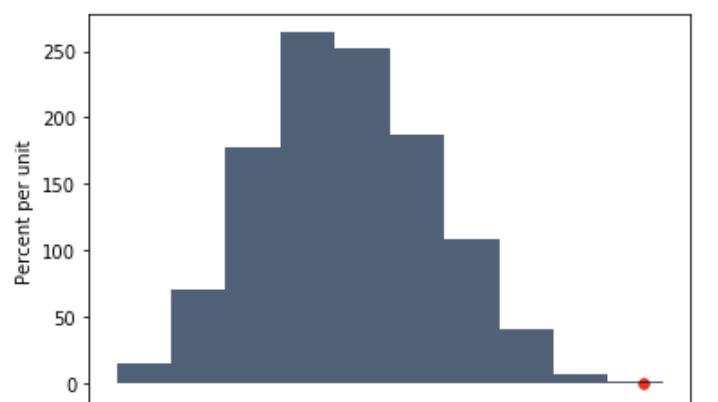
\includegraphics[scale=0.5]{statistics.png}
\end{center}\\
\\ 
\subq{2} Select the best conclusion from the options below: 
\begin{itemize}[label=\bubble]
\item Our data is more consistent with the null hypothesis.
\item Our data is more consistent with the alternative hypothesis.
\item It is impossible to decide given just the histogram above.
\end{itemize}
\solution{Option 2}
\end{enumerate}




    \q{8}{You Studied for these Studies}

\begin{enumerate}

\subq{2} A medical observational study finds a high positive association between drinking coffee and having lung cancer in a group of individuals. Which of the following statements, if true, could present a confounding factor to the study? Choose the best answer.  
\begin{itemize}[label = \bubble]
\item There is a strong positive association between having lung cancer and drinking coffee in this group.
\item There is a strong positive association between drinking coffee and smoking in this group.
\item There is a no association between smoking and having lung cancer in this group.
\item All of the above
\item None of the above 
\end{itemize}
\solution{Option 2}

\subq{2} Researchers decide to test their new disease treatment equipment against their older equipment. However, their new disease equipment requires patients remain hydrated. Researchers select a group of 300 patients for this study; some of the participants will use the new equipment, while the others will use the old equipment. \\
\textbf{Mark all of the following options which} would help control for confounding factors in this study. 
\begin{itemize}[label = \bubble]
\item Requiring patients who are treated with the older equipment remain hydrated.
\item Requiring patients who are treated with the newer equipment remain dehydrated.
\item Assigning patients to groups at random.
\item Assigning different amounts of water randomly to individuals in both groups.
\item None of the above
\end{itemize}
\solution{Option 1 and 3}

\subq{4} A local store is the only umbrella store in a large radius. They decide to test whether or not the quality of their umbrellas impacts their yearly sales. In 2016, their umbrellas were of a very high quality and they sold 1,500 umbrellas. In 2017, their umbrellas were of average quality and they sold 1,000 umbrellas. \\ \\
The store is tempted to explain this phenomenon by claiming that a higher quality of umbrellas causes more sales. As data scientists, however, we are more hesitant to come to this conclusion. Give \textbf{two different specific} alternative explanations that could explain the results of the experiment above. You may \textbf{not} simply claim that this is an observational study. 
\\ \\
1. \\ \\ \\ \\ \\ \\ \\ \\
2. \\ \\ \\ \\ \\ \\ \\ \\
\solution{Two reasons include: \\
1. It didn't rain as much in 2017. No need to buy umbrellas \\
2. People who bought their umbrellas in 2016 didn't need a new one for 2017, so they didn't buy again in 2017. \\
Many options were accepted, if they didn't mention observational study and were specific.}
\end{enumerate}




    \q{8}{P-Value Puzzle}


Define the function {\tt p\_value\_calculation}, which takes in the following 3 arguments: 

\begin{itemize}
\item {\tt sim\_vals} is an array of simulated test statistics under a specific null hypothesis.
\item {\tt observed\_ts} is the value of a test statistic from a specific observed sample.
\item {\tt larger\_alt} is a boolean which is either {\tt True} if only large values of the test statistic above point towards the alternative, and {\tt False} otherwise (small values of the test statistic point towards the alternative).
\end{itemize} 
The function should calculate the P-Value of the {\tt observed\_ts} (observed statistic), with respect to the null hypothesis under which {\tt sim\_vals} was simulated. You may not need all of the lines. 
\\ \\
\lstinline{def p_value_calculation(sim_vals, observed_ts, larger_alt):} \\


\lstinline{	_______________________________________________________________________________} \\ \\


\lstinline{	_______________________________________________________________________________} \\ \\


\lstinline{	_______________________________________________________________________________}\\ \\

\lstinline{        ________________________________________________________________________________} \\ \\


\solution{
\lstinline{def p_value_calculation(sim_vals, observed_ts, larger_alt):} \\
\lstinline{	if larger_alt:} \\ \\
\lstinline{	    return sum(sim_vals >= observed_ts) / len(sim_vals)} \\ \\
\lstinline{	else:}\\ \\
\lstinline{     return sum(sim_vals <= observed_ts) / len(sim_vals)}\
}



    \newpage
    \q{6}{Minimize That!} 

\begin{enumerate}
\subq{2} Assume we have a table, {\tt tbl}, which has two columns. We also have a function which takes in two numbers that represent column indices, and returns the \textbf{negative of the correlation} between the two columns specified by the indices in {\tt tbl}. The first number passed in to the function is the column index for x, and the second number passed in is the column index for y. \\
Assume the correlation between the two columns in {\tt tbl} is .7. If multiple arguments minimize a function, {\tt minimize} randomly chooses one. Which of the following could be the result of calling {\tt minimize} on our function above?
\begin{itemize}[label=\bubble]
\item {\tt array([0,1])}
\item {\tt array([1,0])}
\item Both of the above.
\item None of the above.
\item Cannot tell with this information.
\end{itemize}
\solution{Option 4 -- array([0,0]), and array([1,1]) would have resulted in a correlation of 1, which results in the function returning -1. Since the function returns negative of correlation, this is the smallest value possible.}
\\ \\
\subq{4} We are interested in using {\tt minimize} to find the column with the smallest element in a table {\tt tbl2}. Assume {\tt tbl2} only contains numbers. Define a function {\tt minimized\_fn} which, when passed in to minimize, gives the column index (number) of the column which contains the smallest element in the table. You may not need all of the lines provided below. Afterwards, use your new function to assign {\tt smallest} to the smallest entry in {\tt tbl2}. \\

\lstinline{def minimized_fn(_____________________________________):} \\


\lstinline{	_______________________________________________________________________________} \\ \\


\lstinline{	_______________________________________________________________________________} \\ \\


\lstinline{smallest = ___________________________________________________________________________} \\ \\


\solution{
\lstinline{def minimized_fn(index)} \\


\lstinline{	return min(tbl2.column(index))} \\ \\

\lstinline{smallest = min(tbl2.column(minimize(minimized_fn)))} \\ \\

Minimize expects a function, and returns the arguments of the function which minimize it. The arguments to the function must be numerical. Taking in a table wouldn't make sense. }

\end{enumerate}




    \q{16}{Confidence in Crime}

In 1968, the United States Census Bureau took a large random sample of metropolitan areas and measured their crime rates, measured in proportion per 100,000. The information is encapsulated in a one column table called {\tt crimes}.

\begin{enumerate}

\subq{2} Which of the following pieces of information can we determine given the sample? \textbf{Mark all that apply}.
\begin{itemize}[label=\bubble]
\item The average crime rate in all metropolitan areas in the US in 1968.
\item The approximate distribution of crime rates in metropolitan areas in the US in 1968.
\item The range of crime rates in all metropolitan areas in the US in 1968.
\item None of the above
\end{itemize}  \\
\solution{Option 2}

Assume we bootstrap our sample many times to get an approximate 90\% confidence interval for the average crime rate of the population. The resulting interval is (0.0256, 0.0287).\\

\subq{2} What is the probability that the true average crime rate in the population lies in this interval?
\begin{itemize}[label=\bubble]
\item 100\%
\item 0\%
\item 90\%
\item 95\%
\item None of the above\\
\end{itemize}  
\solution{Option 5, or writing both 100\% or 0\%}

\subq{2} True or False: Approximately 90\% of the population crime rates lie between .0256 and .0286. 
\begin{itemize}[label=\bubble]
\item True
\item False\\
\end{itemize}  
\solution{Option 2 -- Only looking at averages.}

\subq{2} True or False:  Approximately 90\% of the sample crime rates lie between .0256 and .0286. 
\begin{itemize}[label=\bubble]
\item True
\item False\\
\end{itemize}  
\solution{Option 2 -- Only looking at averages}

\subq{3} Suppose the Census Bureau went out and actually sampled two times as many metropolitan areas, so our sample became larger. Would our 90\% confidence interval we calculate using the new data be larger, smaller, around the same size as our original interval, or can we not tell? 
\begin{itemize}[label=\bubble]
\item Larger
\item Smaller
\item Same size
\item Cannot determine \\
\end{itemize}  
\solution{Option 2 -- Sample Size has gotten larger, so by CLT, our width of our confidence interval will becomesmaller}

\subq{3} Assume we want to test the hypothesis that the average population crime rate is .03, with our alternative being that it's not. Give an interval of p-value cutoffs such that we can reject the null hypothesis that the average population crime rate is .03 given our confidence interval above. Explain your answer. Your range should be contained within the interval [0,1]. \\ \\ \\ \\ \\ \\
\solution{[.1,1]. We know that any confidence interval of confidence less than 90\% is contained in the interval we created, so they would reject the null in all of these scenarios. If we increase the confidence, our interval gets larger, and we don't know, then, if our interval will contain .03.}  

\subq{2} Suppose we repeat the process of creating 90\% confidence intervals many times using different samples from the population each time, with the hope of approximately 2,700 intervals containing the true population average crime rate. How many confidence intervals should we create? 
\begin{itemize}[label=\bubble]
\item 900
\item 2,430
\item 2,700
\item 2,850
\item 3,000
\item 3,300
\item None of the above
\end{itemize}  
\solution{Option 5 -- 3000*.9 = 2700, so we should make 3000 CIs.}
\newpage
\end{enumerate} 
    \q{7}{K-Nearest Bobas} \\ 

Tawainese Pearl Milk Tea (also known as boba) is a very common drink on the Berkeley campus. The two main concentrations of boba cafes are on Southside and Downtown Berkeley. Your friend is a Berkeley boba expert. He says that two useful features for classifying boba are the amount of sugar
(x-axis) and the amount of money (y-axis) for a standard black milk tea with pearls. He identifies several boba places for you, but leaves one unknown boba cafe for you to classify, because he hasn't tried it yet. No two boba places have exactly the same features.

You decide to construct a classifier for the unknown boba cafe using all of the known boba cafes as the training set. Note that the x and y axes have different scales.

\begin{center}
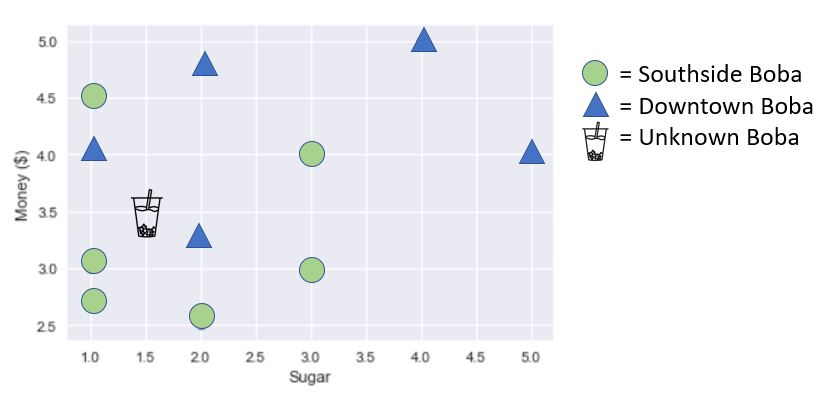
\includegraphics[scale=0.8]{classifiers.JPG}
\end{center}

\begin{enumerate}

\subq{2} Using a 5-nearest neighbor classifier, what would the unknown boba cafe be classified as?
\begin{itemize}[label=\bubble]
\item Southside
\item Downtown
\item Cannot determine
\end{itemize} 

\solution{
	Southside -- 3 southside, 2 downtown
}

\subq{3} What is the problem with using a 4-nearest neighbor classifier for our unknown boba cafe? Provide one possible solution to this problem. \\ \\ \\
\vfill 

\solution{
	It would tie with 2 southside, 2 downtown and then we would need to have a tie breaking scheme
	Any valid tie breaking scheme is accepted -- one could be to choose the class of the point closest, or look at k+1 nearest neighbors when we tie.
}


\subq{2} Every possible pair of feature values for a new boba cafe would be classified as Southside for a 11-nearest neighbor classifier using this training set.
\begin{itemize}[label=\bubble]
\item True
\item False
\item Cannot determine
\end{itemize} 

\solution{
	True. The majority vote will always be southside.
}

\vfill
\end{enumerate}


    \newpage
    \q{0}{(Optional) Data Visualization!}

Draw a data visualization about Data 8.



\end{enumerate}

\end{document}
